\paragraph{Utility} 


\subparagraph{Level 0} 
Common spells \\
\begin{tabular}{ m{2cm}m{3cm}m{8cm}} 
  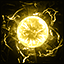
\includegraphics[width=2cm]{../Pictures/Gameplay/Spells/Icon/Lumos_spell_icon.png} & \textbf{Lumos} & Illuminates the tip of the caster's wand, allowing the caster to see in the dark. The spell ends if you cast it again or dismiss it as an action.\\ 
	
\includegraphics[width=2cm]{../Pictures/Gameplay/Spells/Icon/Repario_spell_icon.png} & \textbf{Repario} & Seamlessly repairs broken objects. This spell repairs a single break or tear in an object you touch, such as a broken chain link, two halves of a broken key, a torn cloak, or a leaking wineskin \\ 
	
\includegraphics[width=2cm]{../Pictures/Gameplay/Spells/Icon/Accio_spell_icon.png} & \textbf{Accio} &  Summons an object towards the caster. Describe or name an object that is familiar to you. \\ 
\end{tabular}

\subparagraph{Level 1} 
 Low  spells\\
\begin{tabular}{ m{2cm}m{3cm}m{8cm} } 
 
\includegraphics[width=2cm]{../Pictures/Gameplay/Spells/Icon/Wingardium_spell_icon.png} & \textbf{Wingardium Leviosa} & Makes objects fly, or levitate.   \\ 
	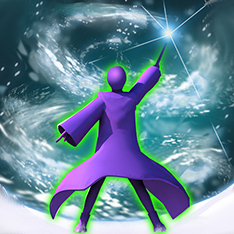
\includegraphics[width=2cm]{../Pictures/Gameplay/Spells/Icon/Fumos_spell_icon.png} & \textbf{Fumos} & It's a charm used to create a defensive cloud of smoke from the wand that hindered visibility. \\  
\end{tabular}

\subparagraph{Level 3} 
Medium  spells\\
\begin{tabular}{ m{2cm}m{3cm}m{8cm} } 
	
\includegraphics[width=2cm]{../Pictures/Gameplay/Spells/Icon/Alomohora_spell_icon.png} & \textbf{Alomohora} & Unlocks doors and other locked objects. \\ 
   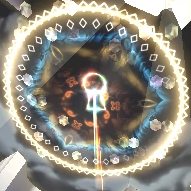
\includegraphics[width=2cm]{../Pictures/Gameplay/Spells/Icon/Colloportus_spell_icon.png} & \textbf{Colloportus} &  Locks doors and all things that can be locked. \\ 
\end{tabular}
	

\subparagraph{Level 5} 
Greater spells\\
\begin{tabular}{ m{2cm}m{3cm}m{8cm} } 
	
\includegraphics[width=2cm]{../Pictures/Gameplay/Spells/Icon/Revelio_spell_icon.png} & \textbf{Revelio} & Reveals secrets about a person or object.  \\ 
	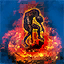
\includegraphics[width=2cm]{../Pictures/Gameplay/Spells/Icon/Transfiguration_spell_icon.png} & \textbf{Transfiguration} &Transform an object into another known object.\\ 
\end{tabular}


\subparagraph{Level 7} 
Superior  spells\\
\begin{tabular}{ m{2cm}m{3cm}m{8cm} } 
	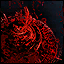
\includegraphics[width=2cm]{../Pictures/Gameplay/Spells/Icon/Apparate_spell_icon.png} & \textbf{Apparate} & Magically transports the caster to another location instantaneously.  \\ 
\end{tabular}

\subparagraph{Level 8} 
Low level spells \\
\begin{tabular}{ m{2cm}m{3cm}m{8cm} } 
  	
\includegraphics[width=2cm]{../Pictures/Gameplay/Spells/Icon/Portkey_spell_icon.png} & \textbf{Portkey} & Turns an object into a portkey.\\ 
\end{tabular}


\pagebreak









